%==============================================================================
\chapter{Theoretical Background}
\label{sec:theory}
%==============================================================================
This chapter will introduce the basic theoretical knowledge needed for the analysis carried out in the following chapters. First, a short overview of the Standard Model of particle physics is given, discussing the fundamental particles and their interactions. Special emphasis is put on the top quark as its properties are pivotal for the four-top-quark process studied in this thesis. The final state and the production channels of the four-top-quark process will be described in the last section of this chapter. \\
It is not common to use S.I. units in elementary particle physics energy, mass and, momenta scales encountered are tiny. The system used instate is known as natural units where [kg,m,s] are replaced by [$\hbar$,$c$,GeV\footnote{GeV is the abbreviation for Giga electron volt where $1\text{eV} = 1.602 \cdot 10^{-19}$ J}]. To simplify the units $\hbar = c = 1$ will be used in this thesis. Thus, all momenta, energies, and masses have the same unit GeV whereas time, and length are given in terms of GeV$^{-1}$.

\section{The Standard Model of Particle Physics}
\label{sec:SM}
\begin{figure}[H]
\centering
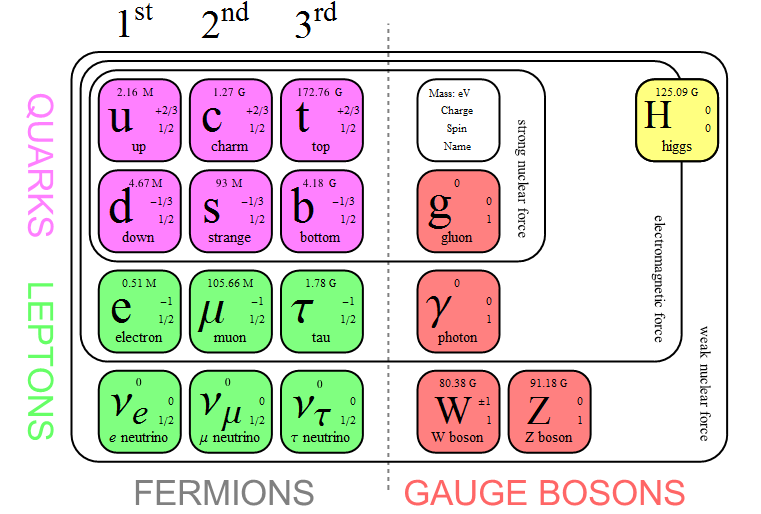
\includegraphics[scale=0.5]{figs/SM.png}
\caption{Schematic depiction of the SM. The masses of the in the SM massive particles are taken from \cite{PDG2020}. The electroweak force is divided into the electromagnetic force and the weak nuclear force. \cite{SMScheme}}
\label{fig:SM}
\end{figure}

The standard model of particle physics (SM) embodies our current understanding of the fundamental constituents of the universe and their interactions. It is a renormalizable quantum field theory constructed from a number of profound theoretical ideas to describe the experimental data observed. As often the case for theories in physics, the SM is guided by the principle of symmetry. Its local gauge symmetry group
\begin{equation*}
SU(3)_{C} \times SU(2)_{L} \times U(1)_{\gamma}
\end{equation*}
consists of the \textit{colour} symmetry group $SU(3)_{C}$ and the symmetry group of the \textit{hypercharge} $SU(2)_{W} \times U(1)_{\gamma}$. The hypercharge and the colour charge are related to the strong nuclear force and the electroweak force respectively. The subscripts $W$ and $\gamma$ indicate that electroweak force is the unification \cite{ModernPP} of the weak nuclear force and the electromagnetic force. $U(n)$ and $SU(n)$ are the unitary and special unitary groups of degree $n$ originating from the group theory structure of the SM \cite{GT}. Therefore, the SM contains two of the fundamental forces of nature. Gravity, which is the third fundamental force can be neglected at the particle level scales. \\
The particles in the SM are elementary particles that means they show no indication of substructure up to the current level of accuracy. All elementary particles can be categorized according to their spin statistics. Particles with half-integer spin obeying the Fermi-Dirac-statics are called \textit{fermions} while particles with integer spin are called \textit{bosons} which obey the Bose-Einstein-statistics \cite{FDStat}. Each particle has an associated antiparticle with the same mass and spin but opposite electrical charge, as well as lepton and baryon numbers. \\
Fermions are further subdivided into \textit{quarks} and \textit{leptons}. Quarks, contrary to leptons, can interact via the strong nuclear force. 
They come in 3 colours and 6 types called \textit{flavors} namely \textit{up}(u), \textit{down}(d), \textit{charm}(c), \textit{bottom}(b), and \textit{top}(t). Mathematically speaking quarks form 3 flavor doublets where the upper component has an electric charge of $Q=\frac{2}{3}$ and the lower an electric charge of $Q=-\frac{1}{3}$. From a physical point of view, this structure is reflected in three \textit{generation} of quarks. The $2^{\text{nd}}$ and $3^{\text{rd}}$ generation quarks have the same quantum number as the quarks from the $1^{\text{st}}$ generation but higher mass. Experimentally it was observed that quarks only exist in bound states of quark-antiquark pairs called \textit{mesons} or three quark or antiquark systems called \textit{baryons}, collectively called \textit{hadrons}. The standard model explains this behavior via \textit{colour confinement}, which states that coloured objects are always confined to colour singlet states and thus are colour neutral. In the case of quarks, the process of confinement is often referred to as \textit{hadronization}. \\
Similarly to quarks, the six leptons of the SM can be sorted into three generations each composed of a doublet. The lepton in the doublet that is electrically neutral and massless\footnote{Neutrinos are massless in the standard model. However, the observation of neutrino oscillations \cite{neutrinoOsci} indicate that they are massive.} is called a \textit{neutrino} ($\nu$). Their massive charge partners are called \textit{electrons} $e$, \textit{muons} $\mu$ and \textit{taus} $\tau$. \\
The forces in the standard model are mediated by \textit{gauge bosons}\footnote{The term ``gauge'' indicates that theories describing the forces are invariant under local gauge transformations \cite{GaugeInv}}. The gauge boson associated with the strong nuclear force is the \textit{gluon}. 
The gluon is a massless particle that carries colour charge. The electroweak force is mediated by three gauge bosons, two massive ones called W$^{\pm}$ and Z bosons, and one massless boson called \textit{photon}. The photon is the only gauge boson that does not carry its own charge and therefore can not self-interact. The strength of each interaction is modelled by energy depending coupling constants. \\
The Standard Model is summarized in Figure \ref{fig:SM}. The only SM particle not yet introduced the Higgs boson discovered in 2012 \cite{Higgs}. It can be interpreted as the excitation of the field predicted by the Higgs mechanism through which elementary particles acquire mass. \\
Even though the standard model is a remarkable achievement of modern science it's not the final answer. It has several shortcomings, for instance it neither provides a candidate for dark matter \cite{DM} nor explains the large matter-antimatter asymmetry in our universe\cite{MAM}.

\newpage  

\section{The Top Quark}
\label{sec:Top}

\begin{figure}[H]
\begin{subfigure}{.5\textwidth}
  \centering
  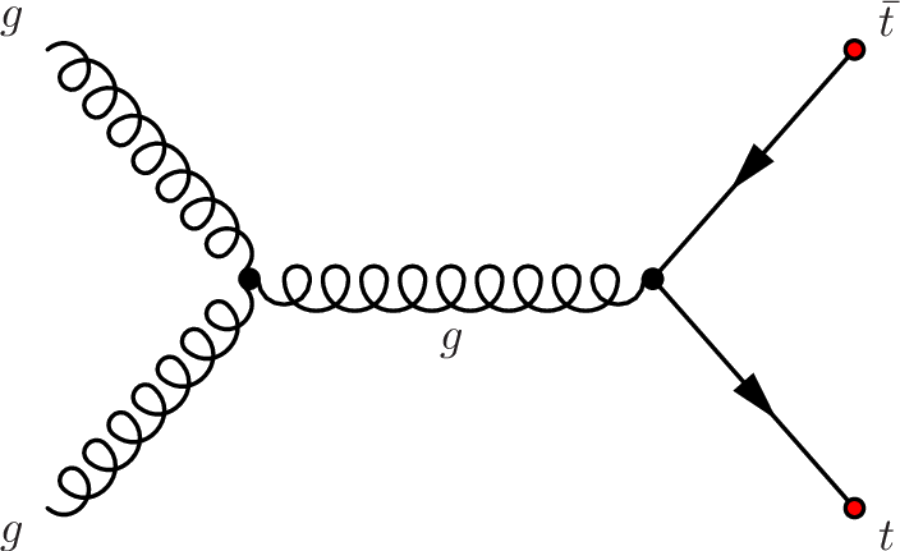
\includegraphics[width=.8\linewidth]{figs/TopPairProduction.png}
  \caption{Top pair production }
  \label{fig:PairProduction}
\end{subfigure}%
\begin{subfigure}{.5\textwidth}
  \centering
  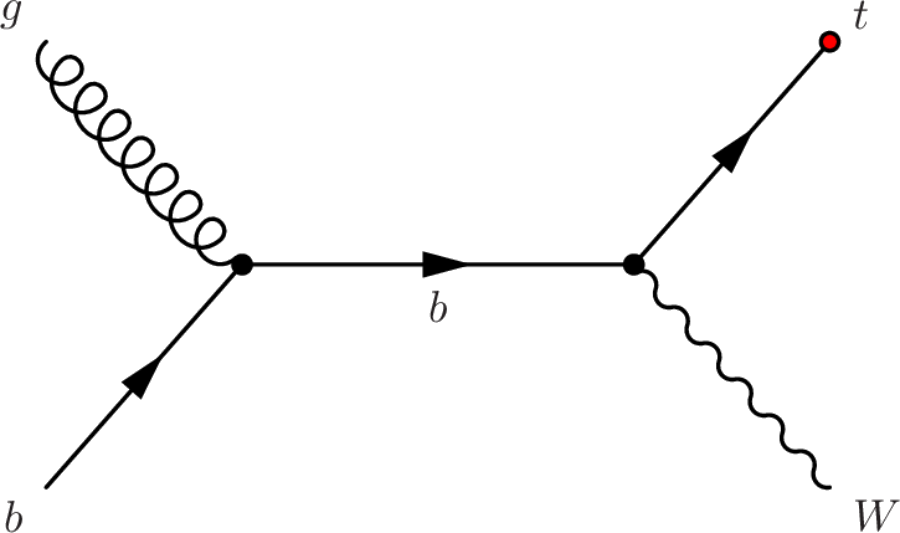
\includegraphics[width=.8\linewidth]{figs/SingleTopProduction.png}
  \caption{Single top production}
  \label{fig:SingleTopProduction}
\end{subfigure}
\caption{The two different categorizes of Top production}
\label{fig:TopProduction}
\end{figure}

The top quark has been first discovered in proton-antiproton collisions at the Fermilab Tevatron Collider in 1995 \cite{TopQuark}. It has a charge of $Q=\frac{2}{3}$ and was observed to be the most massive particle of the Standard Model. The Particle Data group reports a top mass of $m_{t} = 172.76 \pm \SI{0.30}{GeV}$ combing results measured at the Tevatron and the Large Hadron Collider \cite{PDG2020}. Therefore, it is $~40$ times heavier than the next-heaviest quark, the b quark. \\
Owing to its large mass, the lifetime of the top quark $\tau_{\text{t}} \approx 5 \cdot \SI[parse-numbers=false]{10^{-25}}{s}$ \cite{PDG2020} is very short. Consequently, it decays before it can hadronize, since typical time scales for interaction of the strong force are one order of magnitude higher. The decay to a W boson and a quark is governed by the CKM matrix \cite{ModernPP} of the electroweak interaction. Since decays in the same generation are enhanced, the matrix element $|V_{tb}|$ is much bigger than $|V_{ts}|$ and $|V_{tb}|$ resulting in an branching fraction of $BR = 0.90 \pm 0.04$ \cite{PDG2020}.  \\
The production modes of the top quark can be categorized into top-quark pair production and single top production. The processes in which the top is produced in pairs made up the main contribution of events in the discovery of the top quark. This is because processes producing single tops are governed by the electroweak interaction whereas top-antitop pairs are produced via the strong interaction, as can be seen in Figure \ref{fig:TopProduction}. Thus, the first evidence for single top processes was published considerably later in 2006 \cite{singlet}. An advantage of the single top production is that the CKM matrix element $|V_{\text{tb}}|^2$ can be measured directly \cite{CKMtb}.

\newpage

\section{Four-Top-Quark Production}
\label{sec:fourtops}
%The studies carried out in this thesis are related to the official four top-quark analysis of the ATLAS collaboration at $\sqrt{s} = 13$\,TeV [???]. 
The four-top-quark production ($\sigma_{t\bar{t}t\bar{t}}$) is one of the energetically highest processes accessible at the Large Hadron Collider (LHC). The center of mass energy $\sqrt{s}$ required to produce this process has to be at least 4 times the mass of the top quark. The most recent cross-section\footnote{The cross-section $\sigma$ and integrated Luminosity $\mathcal{L}$ will be introduced in Section \ref{sec:LHC}} calculation for proton-proton collisions predict $\sigma_{t\bar{t}t\bar{t}}=11.97^{+18\%}_{-21\%}$ at $\sqrt{s} = \SI{13}{TeV}$ \cite{ttttcross}. The cross-section calculation takes out of all possible production processes only those which are sub-leading in the strong or the electroweak coupling constant into account. Due to its small cross-section is $\sigma_{t\bar{t}t\bar{t}}$ are process which was not observed until now. The cross section of $\sigma_{t\bar{t}t\bar{t}}$ is enhanced in many beyond the Standard Model (BSM) sceneratios such as supersymmerty theories \cite{SuperS} or pair production of scaler gluons \cite{ScalarDing}. \\

\begin{figure}[H]
\begin{subfigure}{.5\textwidth}
  \centering
  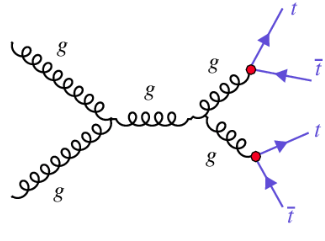
\includegraphics[width=.8\linewidth]{figs/4tproduction1.png}
  \caption{}
  \label{fig:4tproduction1}
\end{subfigure}%
\begin{subfigure}{.5\textwidth}
  \centering
  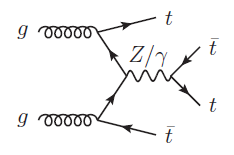
\includegraphics[width=.8\linewidth]{figs/4tproduction2.png}
  \caption{}
  \label{fig:4tproduction2}
\end{subfigure}
\caption{[INTNOTE] Two possible production processes of $t\bar{t}t\bar{t}$ in the SM.}
\label{fig:FourTopProduction}
\end{figure}

The Feynman diagrams of two $t\bar{t}t\bar{t}$ production processes are shown in Figure \ref{fig:FourTopProduction}. As mentioned in Section \ref{sec:Top}, the four top quarks will almost exclusively decay into a b quark and a W boson. The W boson can further decay either hadronically into two quarks or leptonically into a charged lepton and a neutrino, while the b quark will hadronize. The branching ratios for the possible leptonic `$\ell$' and hadronic `$h$' decay combinations are shown in Table \ref{tab:fourtopdecays} where the $\ell \ell hh$ channel is subdivided depending on the charges of the leptons. The $t\bar{t}t\bar{t}$ final state characteristics, therefore, are a high quark multiplicity and 4 b quarks. \\
The analyses of $t\bar{t}t\bar{t}$ carried out by the ATLAS and CMS collaborations are performed either in the one lepton opposite sign channel (1LOS) or in the same sign multilepton channel (SSML). The 1LOS channel considers final states that contain either one lepton or two leptons with opposite charges. The SSML considers final states that contain either two leptons with the same charge or at least 3 leptons. \\
CMS published results in the 1LOS channel and in the SSML channel using $\SI{13}{TeV}$ proton-proton collision data of $\mathcal{L} = \SI{36}{fb}^{-1}$. The quoted observed (expected) upper limits on the $t\bar{t}t\bar{t}$ cross-section are $\SI{48}{fb}$ ($\SI{52}{fb}$) \cite{cross1} and $\SI{41.7}{fb}$ ($\SI{20.8}{fb}$) \cite{cross2} . An updated preliminary result using $\mathcal{L} = \SI{137}{fb}^{-1}$ in the SSML leads to an observed (expected) upper limit of $\SI{22.5}{fb}$ ($\SI{8.5}{fb}$) \cite{cross3}. \\
The results published by the ATLAS collaboration combine the results of both channels and use proton-proton collision data at $\SI{13}{TeV}$ . The observed (expected) upper limit using $\mathcal{L} = \SI{36}{fb}^{-1}$ is $\SI{49}{fb}$ ($\SI{19}{fb}$) \cite{cross4}. The ATLAS analysis that uses the data with $\mathcal{L} = \SI{137}{fb}^{-1}$ is the fist search to claim evidence of four-top-quark production. The $t\bar{t}t\bar{t}$ production cross-section is measured to be $\SI[parse-numbers=false]{24^{+7}_{-6}}{fb}$ \cite{cross5}.

\begin{table}[H]
\centering
\begin{tabular}{|r|r|r|r|r|r|r|}
\toprule
& $hhhh$ & $\ell hhh$ & $\ell \ell hh$ OS & $\ell \ell hh$ SS & $\ell \ell \ell h$ & $\ell \ell \ell \ell$ \\
\midrule
$BR$ & 0.311 & 0.422 & 0.143 & 0.072 & 0.049 & 0.004 \\
\bottomrule
\end{tabular}
\caption{Branching fraction of the different decaying channel of $t\bar{t}t\bar{t}$ following from the decay of four $W$ bosons.}
\label{tab:fourtopdecays}
\end{table}


\section{Three-Top-Quark Production}
\label{sec:Theory3top}

A process that will become important in the analysis carried out in this thesis is the production of three top quarks ($t\bar{t}t$). The most dominant production processes and their branching fractions are shown in Table \ref{tab:BR3t}. All dominant production processes produce $t\bar{t}t$ in association with an additional particle. The most recent calculation of the three top quark cross-section for proton-proton collisions predict $\sigma_{t\bar{t}t} \approx \SI{2}{fb}$ at $\sqrt{s} = \SI{14}{TeV}$ \cite{3t}. \\
The final state of a $t\bar{t}t$ event has at least 3 b-quarks and a center of mass energy higher than 3 times the mass of the top quark. Depending on the decay of the W bosons and the particle produced in association with $t\bar{t}t$, different numbers of leptons, neutrinos, and quarks can be part of the final state composition.

\begin{table}[H]
\centering
\begin{tabular}{|r|r|}
\toprule
Process & branching frac. \\
\midrule
$pp \rightarrow t\bar{t}tW$ & 0.72 \\
$pp \rightarrow t\bar{t}tj$ & 0.19 \\
$pp \rightarrow t\bar{t}tb$ & 0.08 \\
\bottomrule
\end{tabular}
\caption{Dominant background processes and their branching fractions \cite{3t}}
\label{tab:BR3t}
\end{table}

